\chapter{The human microbiome and non-alcoholic fatty liver disease}

\section{Introduction}
Non alcoholic fatty liver disease (NAFLD) has been on the rise along with obesity, affecting a fifth to a third of the North American population \cite{preiss2008non}. Most people with NAFLD remain asymptomatic, however, in up to a third of patients NAFLD can progress to non-alcoholic steatohepatitis (NASH), causing inflammation and scarring in the liver, and decreasing the 5 year survival rate to 67\% \cite{propst1995prognosis}. If we can shed some light on the process by which people progress from NAFLD to NASH, we might be able to find treatments to prevent NASH.

There are several known genetic factors that increase the risk of progression to NASH. The I148M variant of the Patatin-Like Phospholipase Domain Containing 3 gene (PNPLA3) correlates with a 3.2 fold increased risk of NASH from NAFLD when present homozygously, compared to to patients without the variant \cite{sookoian2011meta}. Additionally, mice with a toll-like receptor 4 knockout had lower lipid and injury accumulation markers when fed a methionine/choline-deficient diet which would normally induce steatohepatitis in wild type mice \cite{rivera2007toll}.

On the epigenetic level, genes are differentially methylated in advanced NAFLD compared to mild NAFLD. 11\% of genes are differentially hypomethylated in advanced NAFLD (compared to 3\% hypermethylated), leading to increased expression \cite{murphy2013relationship}. On a hormonal level, estrogen has been shown to inhibit fibrosis in rats \cite{yasuda1999suppressive}. On a metabolite level, Raman et al. found differences in the number of volatile organic compounds detected in patients with NAFLD compared to obese patients without NAFLD \cite{raman2013fecal}. Reactive oxygen species have also been implicated in NASH due to their involvement in the mechanism of steatohepatitis-inducing drugs \cite{berson1998steatohepatitis}.

A 2001 paper performed C-D-xylose-lactulose breath tests and measured tumor necrosis factor alpha levels to determine presence of bacterial overgrowth, and found increased bacterial overgrowth in 22 patients with NASH compared to 23 healthy controls \cite{wigg2001role}. Some papers claim a link between ethanol-producing gut bacteria and NAFLD \cite{zhu2013characterization} \cite{jiang2015dysbiosis}, however, no multiple test correction was performed in these studies.

Several papers have already been published in the literature on the topic of NAFLD and the gut microbiome:

\begin{figure}[h]
\begin{center}
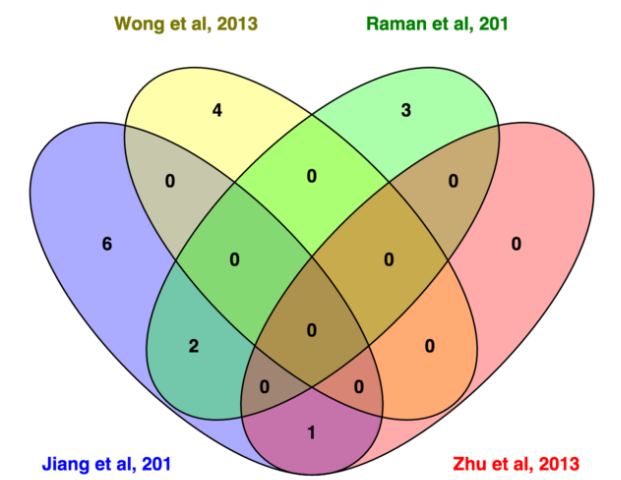
\includegraphics[width=0.7\textwidth]{nafld_papers.png}
\caption{\textbf{Venn diagram of genus found to be differentially abundant by different studies between NASH/NAFLD and healthy controls.} Boursier et al 2015 is not included as they reported a p-value of less than 0.05 for the Bacteroides genus only, which was not reported in any of the other studies. Only 3 out of the 16 genus claimed to be differentially abundant were the same in two studies: Escherichia was found in the Zhu \cite{zhu2013characterization} and Jiang \cite{jiang2015dysbiosis} studies, and Lactobacillus and Oscillibacter were found in the Jiang \cite{jiang2015dysbiosis} and Raman \cite{raman2013fecal} studies.}
\end{center}
\end{figure}

\begin{itemize}
\item Jiang et al, 2015 \cite{jiang2015dysbiosis} compared 53 NAFLD patients with 32 healthy controls

\item Zhu et al, 2013 \cite{zhu2013characterization} compared 16 non-obese controls, 25 obese patients, and 22 NASH patients

\item Raman et al, 2013 \cite{raman2013fecal} compared 30 NAFLD patients with 30 healthy controls

\item Wong et al, 2013 \cite{wong2013molecular} compared 16 NASH patients with 22 healthy controls

\item Boursier et al, 2015 \cite{boursier2016severity} compared 30 patients with F0 or F1 fibrosis to 27 patients with F2 or greater fibrosis, 35 of which had NASH
\end{itemize}

Of these, only Raman et al \cite{raman2013fecal} reported using a multiple test correction.

These five studies do not form a consistent story about the gut microbiome and NAFLD. We hope to run our own analysis rigorously, such that our results are replicable. Additionally, we are running a deeply sequenced metagenomic study, which hasn’t been done in the past.

\FloatBarrier

\section{Methods}
In total, ___ samples were collected from patients with NASH, ___ from patients with SS, and __ from healthy controls. ___ were excluded for ___.
sample data
sample collection
exclusion criteria
DNA extraction

16S rRNA experiment
dna sequencing + barcoding
demultiplexing
quality filtering
clustering
annotation
differential presence (ALDEx

sequencing platform & details
illumina hiseq (check sergio email)
pooling with barcodes

post sequencing processing
demutiplexing
quality filtering (?)

two annotation pipelines
library formation & annotation
assembly & annotation

differential presence analysis with count table
ALDEx
\section{Results}
\section{Discussion}